\documentclass[final]{article}
\usepackage[paperwidth=46.8in,paperheight=35.1in,margin=0.30in]{geometry}
\usepackage[utf8]{inputenc}
\usepackage[T1]{fontenc}
\usepackage[scaled=0.94]{helvet}
\renewcommand{\familydefault}{\sfdefault}
\usepackage{graphicx}
\usepackage{amsmath,amssymb,mathtools}
\usepackage{booktabs,array,tabularx,multirow}
\usepackage[most]{tcolorbox}
\usepackage{xcolor}
\usepackage{ragged2e}
\usepackage{enumitem}
\usepackage{microtype}
\usepackage{tikz}
\usetikzlibrary{arrows.meta,positioning,calc,fit}
\pagestyle{empty}
\setlength{\parindent}{0pt}
\setlength{\parskip}{0.08in}

% ---------- Palette: preserved from NSIA poster ----------
\definecolor{navy}{HTML}{062B63}
\definecolor{navy2}{HTML}{0D3C78}
\definecolor{royal}{HTML}{165A9F}
\definecolor{lightblue}{HTML}{F3F7FC}
\definecolor{lineblue}{HTML}{CAD8EA}
\definecolor{softgreen}{HTML}{EEF8EF}
\definecolor{green}{HTML}{16803A}
\definecolor{softorange}{HTML}{FFF7E6}
\definecolor{orange}{HTML}{C96D00}
\definecolor{softred}{HTML}{FFF1F0}
\definecolor{red}{HTML}{B12020}
\definecolor{graytext}{HTML}{2E3440}
\definecolor{muted}{HTML}{657286}

% ---------- Font helpers ----------
\newcommand{\titlefont}{\fontsize{58}{63}\bfseries\selectfont}
\newcommand{\subtitlefont}{\fontsize{31}{36}\bfseries\selectfont}
\newcommand{\authorfont}{\fontsize{28}{33}\bfseries\selectfont}
\newcommand{\affilfont}{\fontsize{19.5}{23.5}\selectfont}
\newcommand{\bodyfont}{\fontsize{20.0}{24.0}\selectfont}
\newcommand{\smallbody}{\fontsize{17.6}{21.0}\selectfont}
\newcommand{\tinybody}{\fontsize{14.5}{17.0}\selectfont}
\newcommand{\tablefont}{\fontsize{14.7}{17.1}\selectfont}
\newcommand{\captionfont}{\fontsize{13.8}{16.0}\selectfont\color{muted}}

\tcbset{enhanced,boxsep=0.045in,left=0.13in,right=0.13in,top=0.09in,bottom=0.09in,arc=0.06in,outer arc=0.06in,colback=white,colframe=lineblue,boxrule=0.75pt}
\newtcolorbox{sectionbox}[2][]{
  title={#2}, coltitle=white, colbacktitle=navy,
  fonttitle=\fontsize{23.5}{27.5}\bfseries\selectfont,
  attach boxed title to top left={yshift=-0.01in,xshift=0in},
  boxed title style={sharp corners,arc=0.045in,outer arc=0.045in,boxrule=0pt,left=0.12in,right=0.12in,top=0.055in,bottom=0.052in,colback=navy},
  top=0.22in,#1}
\newtcolorbox{claimbox}[1][]{colback=lightblue,colframe=navy2,boxrule=1.05pt,arc=0.09in,left=0.16in,right=0.16in,top=0.10in,bottom=0.10in,#1}
\newtcolorbox{resultbox}[1][]{colback=softgreen,colframe=green,boxrule=1.15pt,arc=0.09in,left=0.16in,right=0.16in,top=0.10in,bottom=0.10in,#1}
\newtcolorbox{warnbox}[1][]{colback=softorange,colframe=orange,boxrule=1.05pt,arc=0.09in,left=0.16in,right=0.16in,top=0.10in,bottom=0.10in,#1}
\newcommand{\mhead}[1]{\textbf{\color{navy}#1}}
\setlist[itemize]{leftmargin=0.22in,itemsep=0.04in,topsep=0.02in,parsep=0pt}

\begin{document}
\bodyfont
\begin{minipage}[t][34.50in][t]{\textwidth}

% ---------- Header ----------
\begin{minipage}[c]{0.105\textwidth}
\centering
\begin{tcolorbox}[width=3.55in,height=2.25in,colback=navy,colframe=navy,arc=0.16in,halign=center,valign=center]
{\fontsize{35}{40}\bfseries\color{white}ECCV}\par
{\fontsize{25}{30}\bfseries\color{white}2026}
\end{tcolorbox}
\end{minipage}\hfill
\begin{minipage}[c]{0.74\textwidth}
  \centering
  {\titlefont\color{navy} Compositional Non-Face Re-Identification Pressure} \\
  {\titlefont\color{navy} under Cumulative Vision Releases}\par
  \vspace{0.16in}
  {\subtitlefont\color{navy2} Auditing the ``leaky bucket'' effect in vision benchmarks}\par
  \vspace{0.22in}
  {\authorfont Tirth Joshi \;\textcolor{muted}{\textbullet}\; Honggang Wang$^{\ast}$} \\
  {\affilfont\color{graytext}Katz School of Science and Health, Yeshiva University, New York, USA}\par
  {\affilfont\texttt{tjoshi1@mail.yu.edu} \quad \texttt{honggang.wang@yu.edu}}
\end{minipage}\hfill
\begin{minipage}[c]{0.13\textwidth}
  \raggedleft
  \begin{tcolorbox}[width=4.15in,height=2.25in,colback=white,colframe=navy2,boxrule=1.4pt,arc=0.16in,halign=center,valign=center]
  {\fontsize{24}{29}\bfseries\color{navy}YESHIVA}\par
  {\fontsize{24}{29}\bfseries\color{navy}UNIVERSITY}\par\vspace{0.06in}
  {\fontsize{15.5}{19}\selectfont\color{muted}Katz School of Science and Health}
  \end{tcolorbox}
\end{minipage}

\vspace{0.05in}
\begin{claimbox}
\centering
\fontsize{20.5}{24.8}\selectfont
\textbf{Main message.} Removing faces does not make identity risk ``reset'' with each new release. Dataset expansions, checkpoints, embeddings, indices, and metadata accumulate as side information. We define \textbf{$vRPI_\alpha$}, prove that true-posterior pressure is non-decreasing under added releases, and show large empirical pressure growth on face-masked Re-ID benchmarks.
\end{claimbox}
\vspace{0.12in}

% ---------- Main 3-column grid ----------
\begin{minipage}[t]{0.292\textwidth}
\vspace{0pt}

\begin{sectionbox}{1. Why Single-Release Privacy Is the Wrong Unit}
\smallbody
Most vision privacy evaluations inspect a dataset or model \emph{in isolation}. Real ecosystems publish artifacts sequentially: more data, new checkpoints/APIs, embeddings, retrieval indices, and sometimes metadata.

\vspace{0.03in}
\mhead{Latent identity and non-face view.}
Let $U\in\{1,\dots,N\}$ index identity, $X$ be a raw observation, and
\[
\widetilde X=\tau(X)
\]
be a non-face transformation. Identity can still remain in clothing, body shape, pose/gait, carried objects, and scene context.

\vspace{0.02in}
\mhead{The compositional question.}
Instead of asking whether one release leaks identity, ask how the posterior
\[
\Pr(U\mid Z_{1:T})
\]
sharpens as releases accumulate. The operational target is Bayes-optimal guessing:
\[
P_{\mathrm{guess}}(U\mid Z_{1:T})
=\mathbb E\!\left[\max_u \Pr(U=u\mid Z_{1:T})\right].
\]
\end{sectionbox}

\vspace{0.12in}
\begin{sectionbox}{2. Release-as-Channel Formulation}
\centering
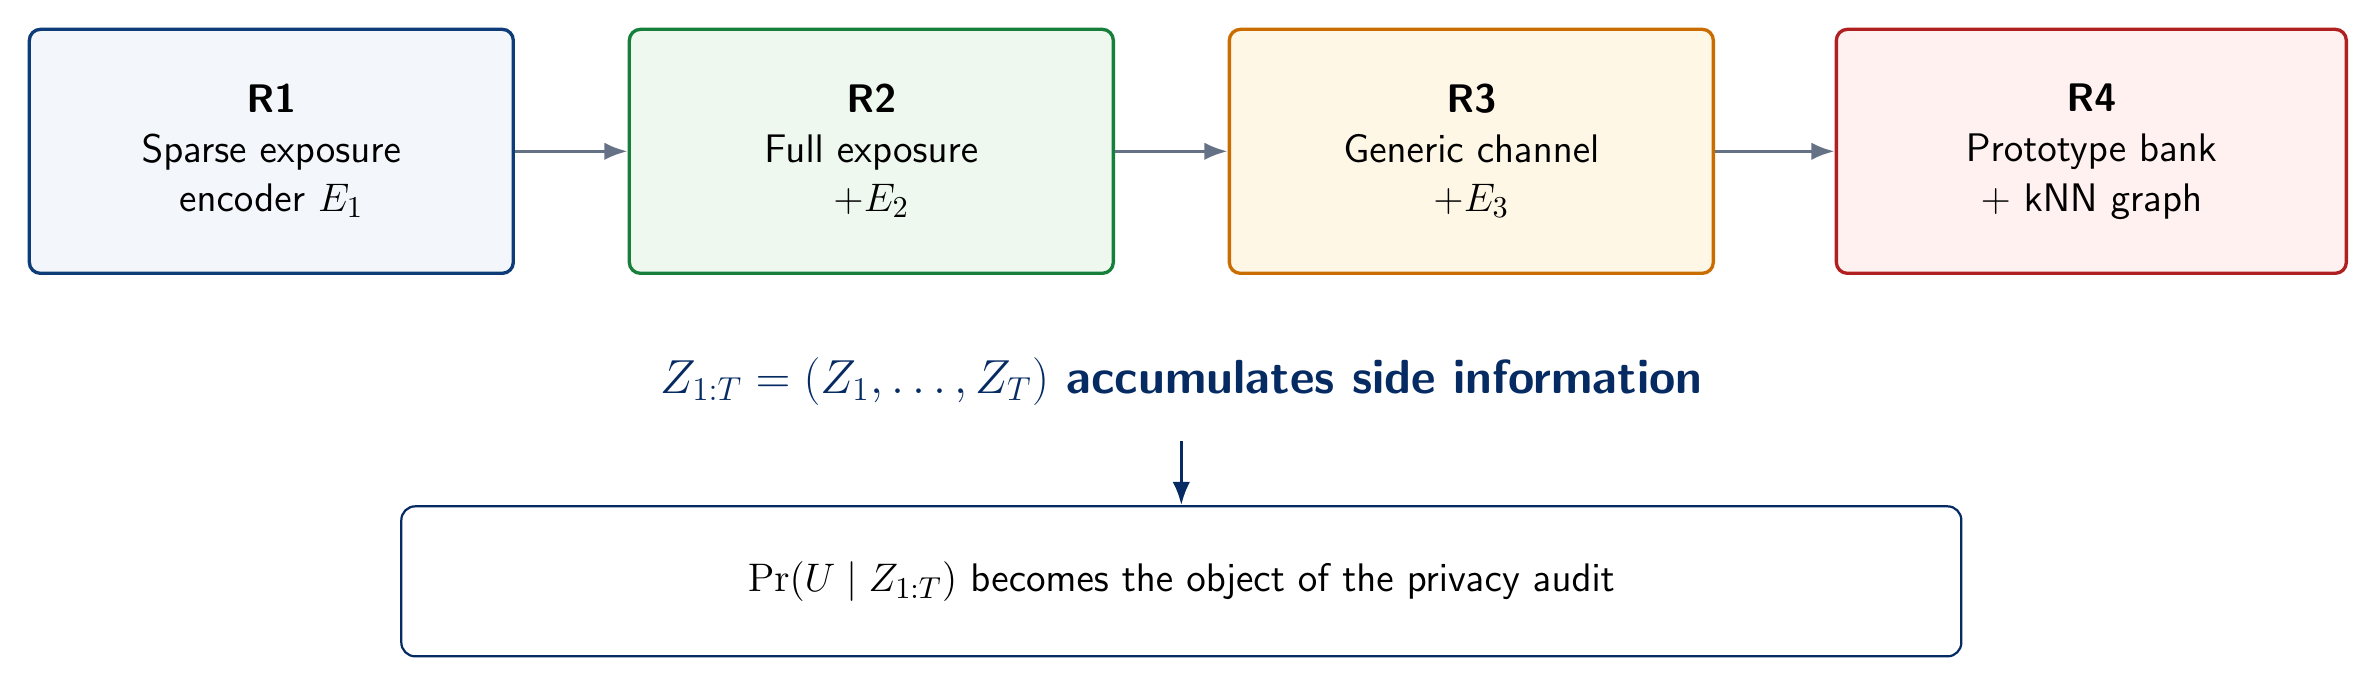
\begin{tikzpicture}[x=1in,y=1in,>=Latex, every node/.style={font=\fontsize{15.5}{18}\selectfont}]
\node[draw=navy2,very thick,rounded corners=4pt,fill=lightblue,minimum width=2.42in,minimum height=1.22in,align=center] (r1) at (0,0) {\textbf{R1}\\Sparse exposure\\encoder $E_1$};
\node[draw=green,very thick,rounded corners=4pt,fill=softgreen,minimum width=2.42in,minimum height=1.22in,align=center] (r2) at (3.0,0) {\textbf{R2}\\Full exposure\\$+E_2$};
\node[draw=orange,very thick,rounded corners=4pt,fill=softorange,minimum width=2.42in,minimum height=1.22in,align=center] (r3) at (6.0,0) {\textbf{R3}\\Generic channel\\$+E_3$};
\node[draw=red,very thick,rounded corners=4pt,fill=softred,minimum width=2.55in,minimum height=1.22in,align=center] (r4) at (9.1,0) {\textbf{R4}\\Prototype bank\\+ kNN graph};
\draw[->,very thick,color=muted] (r1)--(r2);
\draw[->,very thick,color=muted] (r2)--(r3);
\draw[->,very thick,color=muted] (r3)--(r4);
\node[align=center,text=navy,font=\fontsize{16.5}{20}\bfseries] at (4.55,-1.15) {$Z_{1:T}=(Z_1,\ldots,Z_T)$ accumulates side information};
\node[draw=navy,thick,rounded corners=5pt,fill=white,minimum width=7.8in,minimum height=.75in,align=center] (post) at (4.55,-2.15) {$\Pr(U\mid Z_{1:T})$ becomes the object of the privacy audit};
\draw[->,very thick,color=navy] (4.55,-1.45)--(post.north);
\end{tikzpicture}

\vspace{0.02in}
{\captionfont Each disclosure is modeled as a channel $Z_t\sim K_t(\cdot\mid\widetilde X)$. The framework is release-sequence aware rather than tied to one Re-ID model or anonymizer.}
\end{sectionbox}

\vspace{0.12in}
\begin{sectionbox}{3. $vRPI_\alpha$: Metric and Core Theory}
\smallbody
\mhead{Rényi pressure index.} For $\alpha>1$, using Arimoto conditional Rényi entropy,
\[
\boxed{vRPI_\alpha(T)=\log N-H_\alpha(U\mid Z_{1:T})}.
\]
For a uniform prior, $\log N$ is maximal identity uncertainty, so $vRPI_\alpha$ measures how much anonymity has been eroded by cumulative releases.

\vspace{0.03in}
\begin{tcolorbox}[colback=lightblue,colframe=navy2,left=.10in,right=.10in,top=.07in,bottom=.07in]
\textbf{Theorem 1: monotonicity on the true posterior}
\[
H_\alpha(U\mid Z,W)\le H_\alpha(U\mid Z)
\Longrightarrow
vRPI_\alpha(T+1)\ge vRPI_\alpha(T).
\]
Added side information cannot restore identity uncertainty.
\end{tcolorbox}

\vspace{0.03in}
\begin{tcolorbox}[colback=softgreen,colframe=green,left=.10in,right=.10in,top=.07in,bottom=.07in]
\textbf{Theorem 2: operational guessing bridge}
\[
P_{\mathrm{guess}}(U\mid Z)
\le
\exp\!\left(\frac{1-\alpha}{\alpha}H_\alpha(U\mid Z)\right).
\]
Thus higher pressure corresponds to a smaller effective anonymity set and stronger identity inference.
\end{tcolorbox}

\vspace{0.02in}
\mhead{Choosing $\alpha$.} $\alpha=2$ is the recommended stable default; $\alpha=5$ or $10$ emphasizes high-confidence / worst-case posterior concentration and should be paired with calibration diagnostics.

\vspace{0.04in}
\mhead{Additional guarantees.}
\begin{itemize}
  \item \textbf{Ideal additivity benchmark.} If releases are conditionally independent given identity, Sibson information factorizes and gives an additive upper benchmark on pressure:
  \[
  vRPI_\alpha(T)\le \sum_{t=1}^{T} I^{\mathrm S}_\alpha(U;Z_t).
  \]
  \item \textbf{Ablation monotonicity.} If $\tau_B$ is a post-processing of $\tau_A$, then removing information cannot increase pressure:
  \[
  vRPI_\alpha^A(T)\ge vRPI_\alpha^B(T).
  \]
  \item \textbf{Plug-in stability.} If the estimated posterior is close in expected $\ell_1$ error, the estimated $vRPI_\alpha$ changes continuously, with an explicit logarithmic error bound.
\end{itemize}
\end{sectionbox}
\end{minipage}\hfill
% ---------- Middle column ----------
\begin{minipage}[t]{0.388\textwidth}
\vspace{0pt}

\begin{sectionbox}{4. Main Empirical Result on Market-1501-$\tau$}
\begin{resultbox}
\smallbody
\textbf{The dominant leak is exposure expansion.} From R1 to R2, retrieval attacker A0 jumps from $P_{\mathrm{guess}}=0.288$ to $0.749$ and $vRPI_2=4.332$ to $6.212$. A3 rises from $0.407$ to $0.706$. R4 then shows that publishable artifacts themselves create exploitable leakage pathways.
\end{resultbox}
\vspace{0.045in}
\tablefont
\renewcommand{\arraystretch}{1.14}
\setlength{\tabcolsep}{5.0pt}
\resizebox{\linewidth}{!}{%
\begin{tabular}{llccl}
\toprule
\textbf{Release} & \textbf{Attacker} & $\mathbf{P_{guess}}$ & $\mathbf{vRPI_2}$ & \textbf{Interpretation}\\
\midrule
R1 & A0 & .2883 & 4.3319 & Sparse exposure baseline\\
R2 & A0 & \textcolor{green}{\textbf{.7491}} & \textcolor{green}{\textbf{6.2119}} & Dominant exposure-expansion jump\\
R3 & A0 & .7529 & 5.9271 & Generic channel; calibrated fusion\\
R4 & A2 & \textcolor{red}{\textbf{.7519}} & \textcolor{red}{\textbf{6.3572}} & Prototype/index specialist\\
R4 & A0-Graph & .7366 & 5.6697 & kNN-graph pathway\\
\bottomrule
\end{tabular}}
\vspace{0.02in}

{\captionfont Mean over 3 seeds. A3 independently shows the same R1$\rightarrow$R2 pattern ($P_{\mathrm{guess}}$: .407$\rightarrow$.706; $vRPI_2$: 4.723$\rightarrow$5.940). Empirical plug-in estimates can fluctuate with attacker/calibration even though Theorem 1 is a true-posterior statement.}
\end{sectionbox}

\vspace{0.12in}
\begin{sectionbox}{5. Release Trend: The R1$\rightarrow$R2 Jump Dominates}
\centering
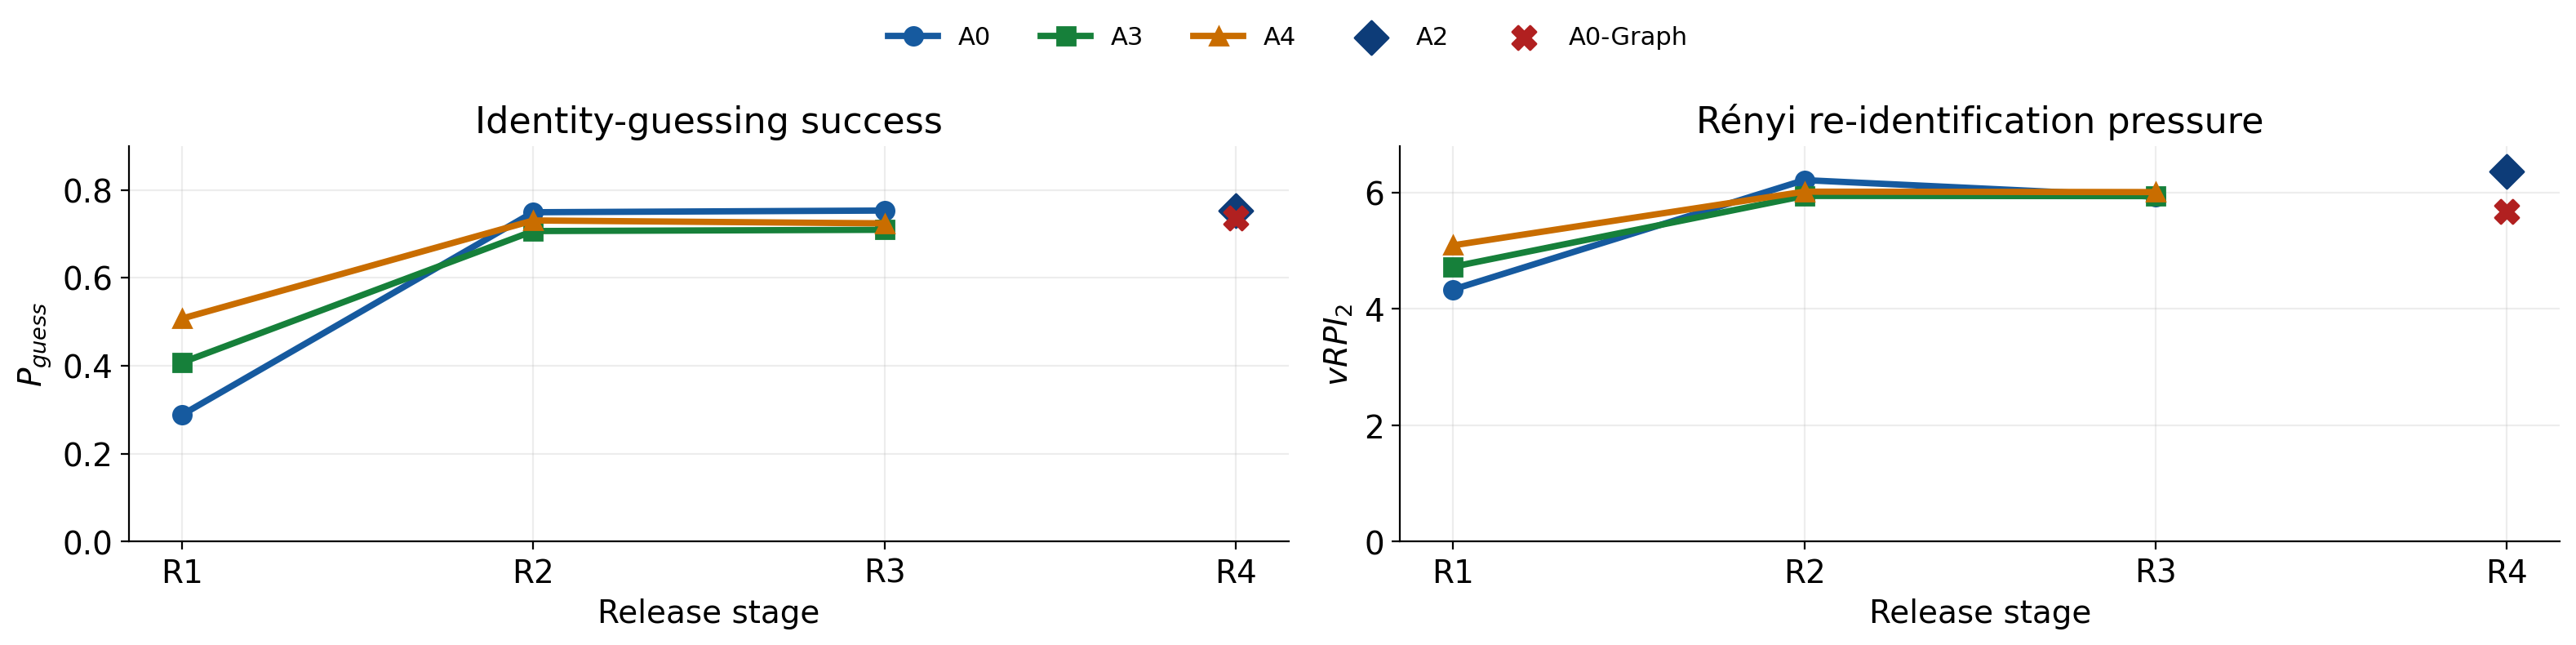
\includegraphics[width=0.94\linewidth]{assets/fig_release_trends.png}
\vspace{-0.05in}

{\captionfont The exposure expansion is the clearest compositional effect. R2$\rightarrow$R3 is stable under validation-tuned fusion and temperature scaling. R4 demonstrates artifact-specific leakage through the prototype/index specialist and graph-exploiting attacker.}
\end{sectionbox}

\vspace{0.12in}
\begin{sectionbox}{6. Replication + Non-Face Stress Test}
\centering
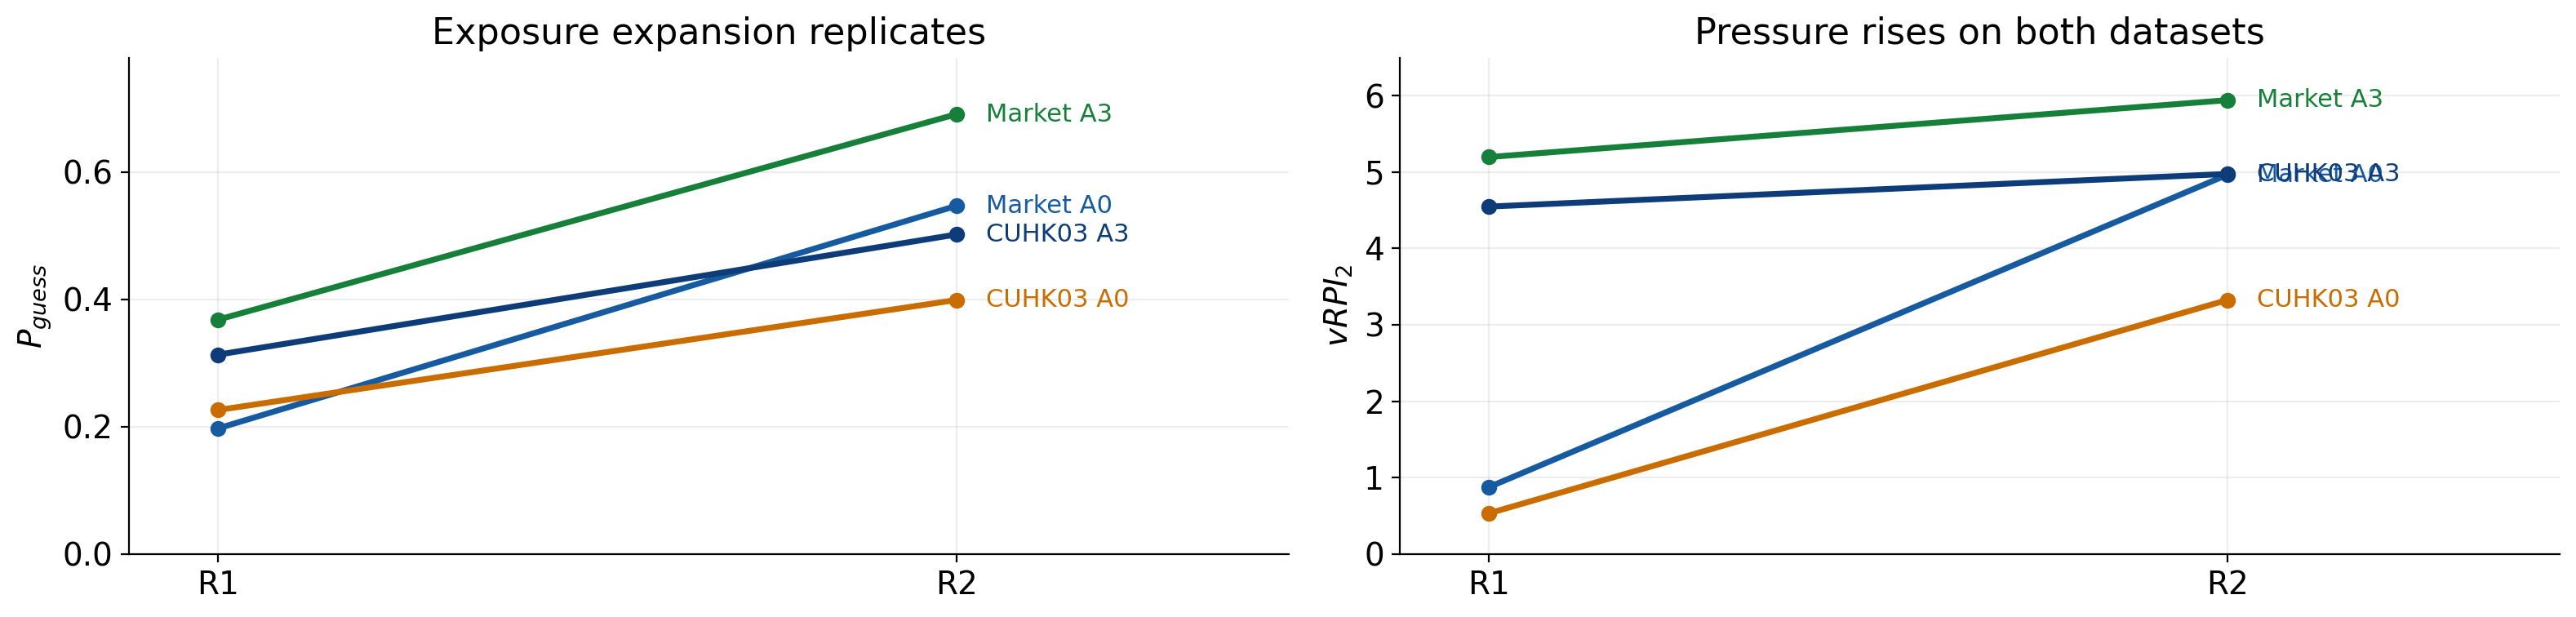
\includegraphics[width=0.94\linewidth]{assets/fig_replication.png}
\vspace{-0.04in}

\smallbody
\begin{minipage}[t]{0.49\linewidth}
\mhead{CUHK03-$\tau$ replication.} A lighter paired protocol still yields a positive R1$\rightarrow$R2 increase for both retrieval (A0) and nonlinear-probe (A3) attackers on Market and CUHK03. The absolute magnitudes are not compared across protocols; the paired direction is the claim.
\end{minipage}\hfill
\begin{minipage}[t]{0.49\linewidth}
\mhead{Masking ablation.} Sweeping top-region masking from 0\% to 40\% leaves pressure essentially flat: A0 $vRPI_2\in[4.87,4.91]$, A3 $vRPI_2\in[5.83,5.88]$. Even at 40\% masking, $P_{\mathrm{guess}}\ge .51$ (A0) and $\ge .64$ (A3).
\end{minipage}

\vspace{0.04in}
\begin{warnbox}
\smallbody
\textbf{Important scope.} The top-region mask is a controlled proxy, not a realistic detector-based or generative anonymizer. The result shows persistent non-face signal under aggressive region removal; it does not claim that all anonymization methods fail.
\end{warnbox}
\end{sectionbox}

\end{minipage}\hfill
% ---------- Right column ----------
\begin{minipage}[t]{0.292\textwidth}
\vspace{0pt}

\begin{sectionbox}{7. Experimental Protocol and Attacker Ladder}
\smallbody
\mhead{Dataset.} Main experiment: Market-1501 training identities, $N=751$, with the top 20\% of each image masked (Market-1501-$\tau$). Images are split into exposure, gallery, query, and held-out validation pools over the same closed-world label space.

\vspace{0.03in}
\mhead{What counts as a release?}
\begin{itemize}
  \item \textbf{R1:} encoder $E_1$ trained on sparse exposure.
  \item \textbf{R2:} add $E_2$ trained on full exposure; cumulative feature state.
  \item \textbf{R3:} add generic ImageNet-pretrained ResNet-50 $E_3$.
  \item \textbf{R4:} publish an identity prototype bank and a kNN graph derived from the R3 gallery.
\end{itemize}

\vspace{0.02in}
\mhead{Attacker ladder.}
\begin{itemize}
  \item \textbf{A0} black-box retrieval with identity-level posterior aggregation.
  \item \textbf{A1} linear probe.
  \item \textbf{A2} prototype-index specialist (R4).
  \item \textbf{A3} MLP / nonlinear probe.
  \item \textbf{A4} white-box fine-tuning (R1--R3).
\end{itemize}
Every attacker maps scores into a posterior over the same identity universe before entropy computation.
\end{sectionbox}

\vspace{0.12in}
\begin{sectionbox}{8. Diagnostics: Dependence, Calibration, Priors}
\smallbody
\mhead{Dependence overlap.} Conditional independence gives an ideal additive benchmark, not a claim about real CV releases. On Market,
\[
\Delta_{\mathrm{corr},2}
=\sum_t \widehat{vRPI}_2(Z_t)
-\widehat{vRPI}_2(Z_{1:T})
=0.304>0,
\]
quantifying redundancy among correlated release channels.

\vspace{0.03in}
\mhead{Temperature calibration.} Across $\theta\in\{.025,.05,.1,.2,.5,1.0\}$, absolute pressure changes, but
\[
\Delta vRPI_2(R2-R1)>0
\]
throughout: A0 spans $[.781,4.100]$ and A3 $[.567,.677]$.

\vspace{0.03in}
\mhead{Non-uniform identity priors.} For a Zipf$(s)$ prior, normalize by prior entropy:
\[
vRPI_\alpha^{\pi}(T)
=H_\alpha(U)-H_\alpha(U\mid Z_{1:T}).
\]
The R1$\rightarrow$R2 increment shrinks from $3.818$ at $s=0$ to $.123$ at $s=1.5$, because a concentrated prior leaves less anonymity to erode.
\end{sectionbox}

\vspace{0.12in}
\begin{sectionbox}{9. What the Framework Adds}
\smallbody
\mhead{Not another Re-ID model.} $vRPI_\alpha$ audits the privacy pressure induced by releases; rank/mAP remains a retrieval-utility metric. The two answer different questions.

\vspace{0.03in}
\mhead{Not a replacement for maximal leakage or DP.} Maximal leakage optimizes adversarial gain at the channel level, while DP supplies worst-case stability guarantees. $vRPI_\alpha$ instead fixes the vision identity task and measures posterior concentration over a release sequence.

\vspace{0.03in}
\mhead{Governance implication.} Privacy review should happen at the \textbf{sequence level}: evaluate planned dataset/model/index disclosures together, minimize unnecessary metadata, and treat high-leverage artifacts such as embedding dumps, prototype banks, and indices as privacy-relevant releases.

\vspace{0.03in}
\vspace{0.03in}
\mhead{Positioning against common criteria.}
\tablefont
\renewcommand{\arraystretch}{1.12}
\resizebox{\linewidth}{!}{%
\begin{tabular}{lll}
\toprule
\textbf{Measure} & \textbf{Object measured} & \textbf{Sequence-aware?}\\
\midrule
Rank/mAP & Retrieval ranking quality & No\\
$P_{\mathrm{guess}}$ & Bayes posterior maximum & Yes, on $Z_{1:T}$\\
$vRPI_\alpha$ & Rényi posterior concentration & \textbf{Yes}\\
Maximal leakage & Worst-case channel gain & Channel-level\\
DP / attribute inference & Worst-case stability / bound & Via composition\\
\bottomrule
\end{tabular}}

\vspace{0.04in}
\begin{tcolorbox}[colback=softgreen,colframe=green,left=.10in,right=.10in,top=.07in,bottom=.07in]
\smallbody
\textbf{Release hygiene, not surveillance.} The intended use is governance: audit successive disclosures before publication, limit high-leverage artifacts, and minimize unnecessary metadata exposure.
\end{tcolorbox}

\vspace{0.03in}
\mhead{Limitations.}
\begin{itemize}
  \item Closed-world image benchmarks; broader datasets, video, larger scale, and open-set evaluation remain future work.
  \item Top-region masking is a controlled proxy rather than realistic anonymization.
  \item $vRPI_\alpha$ is an audit statistic, not a mitigation method.
\end{itemize}
\end{sectionbox}

\end{minipage}

\vspace{0.14in}
\begin{sectionbox}[height=3.65in]{10. Final Contribution, Empirical Signal, and Limitation}
\begin{minipage}[t]{0.318\linewidth}
\begin{tcolorbox}[height=3.45in,colback=lightblue,colframe=navy2,left=0.14in,right=0.14in,top=0.12in,bottom=0.10in]
{\fontsize{27}{32}\bfseries\color{navy}Contribution}\par\vspace{0.06in}
{\fontsize{19.8}{24.2}\selectfont
A \textbf{release-sequence privacy formalism} and $vRPI_\alpha$, derived from Arimoto conditional Rényi entropy.\par\vspace{0.10in}
\textbf{Theory:} monotonicity under added side information, a Bayes-guessing bridge, an ideal additive benchmark, ablation monotonicity, and plug-in stability.}
\end{tcolorbox}
\end{minipage}\hfill
\begin{minipage}[t]{0.318\linewidth}
\begin{tcolorbox}[height=3.45in,colback=softgreen,colframe=green,left=0.14in,right=0.14in,top=0.12in,bottom=0.10in]
{\fontsize{27}{32}\bfseries\color{navy}Empirical signal}\par\vspace{0.06in}
{\fontsize{19.8}{24.2}\selectfont
On face-masked Market-1501, \textbf{exposure expansion causes the dominant jump}: A0 $P_{\mathrm{guess}}$ rises .288$\rightarrow$.749 and $vRPI_2$ rises 4.332$\rightarrow$6.212.\par\vspace{0.10in}
CUHK03 preserves the paired R1$\rightarrow$R2 direction, while prototype/index and kNN-graph releases create artifact-specific leakage pathways.}
\end{tcolorbox}
\end{minipage}\hfill
\begin{minipage}[t]{0.318\linewidth}
\begin{tcolorbox}[height=3.45in,colback=softorange,colframe=orange,left=0.14in,right=0.14in,top=0.12in,bottom=0.10in]
{\fontsize{27}{32}\bfseries\color{navy}Limitation}\par\vspace{0.06in}
{\fontsize{19.8}{24.2}\selectfont
The evaluation is intentionally theory-aligned and closed-world. $vRPI_\alpha$ is an \textbf{audit statistic, not a mitigation}.\par\vspace{0.10in}
Next: \textbf{open-set posteriors, realistic anonymizers, more datasets/video, and longer real release sequences} that better match evolving benchmark ecosystems.}
\end{tcolorbox}
\end{minipage}
\end{sectionbox}

\vfill
\vspace{0.06in}
\begin{tcolorbox}[enhanced,colback=navy,colframe=navy,boxrule=0pt,arc=0in,outer arc=0in,left=0.22in,right=0.22in,top=0.09in,bottom=0.09in]
\begin{minipage}[c]{0.30\textwidth}
  {\fontsize{18}{22}\bfseries\color{white} Tirth Joshi \;\textcolor{lineblue}{\textbullet}\; Honggang Wang} \\
  {\fontsize{16}{20}\selectfont\color{white}Katz School of Science and Health, Yeshiva University}
\end{minipage}\hfill
\begin{minipage}[c]{0.46\textwidth}
  \centering
  {\fontsize{19}{23}\bfseries\color{white} Compositional Non-Face Re-Identification Pressure under Cumulative Vision Releases}\par
  {\fontsize{16}{19}\selectfont\color{white}\texttt{tjoshi1@mail.yu.edu}}
\end{minipage}\hfill
\begin{minipage}[c]{0.18\textwidth}
  \raggedleft
  {\fontsize{18}{22}\bfseries\color{white}ECCV 2026}\par
  {\fontsize{14.5}{18}\selectfont\color{lineblue}$^{\ast}$Corresponding author}
\end{minipage}
\end{tcolorbox}

\end{minipage}
\end{document}
